% !TEX TS-program = xelatex
% !TEX encoding = UTF-8

% This is a simple template for a XeLaTeX document using the "article" class,
% with the fontspec package to easily select fonts.

 % use larger type; default would be 10pt
\documentclass[12pt,twopage]{book}
\usepackage[czech]{babel}
\usepackage{ucs}
% Unicode support for LaTeX character names (accents, European chars, etc)
\usepackage{fontenc}
\usepackage{xltxtra,fontspec,xunicode}

% syntax highlight
\usepackage{listings}
\usepackage{xcolor}

\usepackage{cleveref}


% colors
\definecolor{javared}{rgb}{0.0,0.4,0.8} % for strings
\definecolor{javagreen}{rgb}{0.55,0.55,0.55} % comments
\definecolor{javapurple}{rgb}{0.8,0.4,0,0} % keywords
\definecolor{javadocblue}{rgb}{0.45,0.45,0.45} % javadoc
% define backgroundcolor
\definecolor{bggray}{rgb}{0.97, 0.97, 0.99}

\frenchspacing



\definecolor{bublina1}{rgb}{0.75,0.75,0.75} % for strings
\definecolor{bublina2}{rgb}{0.33,0.66,0.99} % comments
\usepackage[dvips]{hyperref}


\hypersetup{
    bookmarks=true,         % show bookmarks bar?
    unicode=false,          % non-Latin characters in Acrobat’s bookmarks
    pdftoolbar=true,        % show Acrobat’s toolbar?
    pdfmenubar=true,        % show Acrobat’s menu?
    pdffitwindow=false,     % window fit to page when opened
    pdfstartview={FitH},    % fits the width of the page to the window
    pdftitle={Processing 1.0},    % title
    pdfauthor={Kryštof Pešek},     % author
    pdfsubject={Processing 1.0},   % subject of the document
    pdfcreator={Kryštof Pešek},   % creator of the document
    pdfproducer={AMU}, % producer of the document
    pdfkeywords={processing} {příručka} {kof}, % list of keywords
    pdfnewwindow=true,      % links in new window
    colorlinks=true,       % false: boxed links; true: colored links
    linkcolor=bublina2,          % color of internal links
    citecolor=green,        % color of links to bibliography
    filecolor=magenta,      % color of file links
    urlcolor=red           % color of external links
}


\usepackage{makeidx}
\usepackage{index}     % balík pro indexování
\usepackage[all]{hypcap}


\usepackage{graphicx} % support the \includegraphics command and options
\usepackage{verbatim}

%\usepackage[utf8x]{inputenc}


%uvozovky cs
\renewcommand\uv[1]{\quotedblbase #1\textquotedblleft}%


\usepackage[xindy]{glossaries}


\usepackage{marginnote}
\usepackage[textsize=footnotesize,textwidth=3cm]{todonotes}
\setlength{\marginparwidth}{3.1cm}

\newcommand{\oddil}[1]{\section{#1}\label{sec:#1}}
\newcommand{\pododdil}[1]{\subsection{#1}\label{subsec:#1}}
%%% BUBLINY

\usepackage{setspace}

\newcommand{\bublina}[1]{\todo[color=bublina1]{\em #1}}
\newcommand{\otazka}[1]{\todo[color=bublina2]{\em #1}}
\newcommand{\kof}[1]{\todo[color=javadocblue]{\em #1}}


\newcommand{\klavesy}[1]{\textsc{\em #1}}

\newcommand{\slovnik}[1]{\textbf{\gls{#1}}\index{#1}}
\newcommand{\Slovnik}[1]{\textbf{\Gls{#1}}\index{#1}}
\newcommand{\slovnikpl}[1]{\textbf{\glspl{#1}}\index{#1}}
\newcommand{\Slovnikpl}[1]{\textbf{\Glspl{#1}}\index{#1}}

\newcommand{\definice}[2]{\newglossaryentry{#1}{ }{ name={#1},description{#2} } }

\newcommand{\vyraz}[1]{\textit{\gls{#1}}\index{#1}}




%\newcounter{todocounter}
%\newcommand{\bokem}[2][]
%{\stepcounter{todocounter}\todo[#1]{\thetodocounter: #2}}




% pomocné příkazy
%\def\cindex{\index*[cmnd]}        % zařazení do rejstříku příkazů
%\newcommand{\hla}[1]{\textit{#1}} % pro vysvětlení pojmu


% lsset, kód jak vypadá
% Add your keywords here,  and have this in a separate file
% and include it in your preamble
\lstset{emph={abs, acos, alpha, ambient, ambientLight, append, applyMatrix, arc, arraycopy, asin, atan, atan2, background, beginCamera, beginRecord, beginShape, bezier, bezierDetail, bezierPoint, bezierTangent, bezierVertex, binary, blend, blendColor, blue, box, brightness, camera, ceil, colorMode, concat, constrain, cos, createFont, createGraphics, createImage, createWriter, cursor, curve, curveDetail, curvePoint, curveTightness, curveVertex, day, degrees, delay, directionalLight, dist, draw, ellipse, ellipseMode, emissive, endCamera, endRecord, endShape, exit, exp, expand, fill, filter, floor, frustum, get, green, hex, hint, hour, hue, image, imageMode, join, keyReleased, keyTyped, lerp, lerpColor, lightFalloff, lights, lightSpecular, line, link, loadBytes, loadFont, loadImage, loadPixels, loadStrings, log, loop, mag, map, match, max, millis, min, minute, modelX, modelY, modelZ, month, mouseClicked, mouseDragged, mouseMoved, mouseReleased, nf, nfc, nfp, nfs, noCursor, noFill, noise, noiseDetail, noiseSeed, noLoop, norm, normal, noSmooth, noStroke, noTint, open, openStream, ortho, param, perspective, list, beginDraw, endDraw, blend, copy, mask, set, point, pointLight, popMatrix, pow, printCamera, printMatrix, printProjection, close, flush, print, println, pushMatrix, quad, radians, random, randomSeed, rect, rectMode, red, redraw, resetMatrix, reverse, rotate, rotateX, rotateY, rotateZ, round, saturation, save, saveBytes, saveFrame, saveStrings, scale, screenX, screenY, screenZ, second, setup, shininess, shorten, sin, size, smooth, sort, specular, sphere, sphereDetail, splice, split, splitTokens, spotLight, sq, sqrt, status, str, charAt, equals, indexOf, length, substring, toLowerCase, toUpperCase, stroke, strokeCap, strokeJoin, strokeWeight, subset, tan, text, textAlign, textAscent, textDescent, textFont, textLeading, textMode, textSize, texture, textureMode, textWidth, tint, translate, triangle, trim, unbinary, unhex, unhint, updatePixels, vertex, year, keyPressed, mousePressed, frameRate}
, emphstyle={\color{javapurple}}%
}%



\lstset{
language=Java,
basicstyle=\footnotesize\ttfamily,
frame=none,
framesep=10pt,
keywordstyle=\color{javapurple},
stringstyle=\color{javared},
commentstyle=\color{javagreen},
morecomment=[s][\color{javadocblue}]{/**}{*/},
stepnumber=2,
numbersep=10pt,
tabsize=4,
showspaces=false,
showstringspaces=false,
backgroundcolor=\color{bggray}
literate = {{š}{{\v s}}1 {č}{{\v c}}1 {ž}{{\v z}}1 {ř}{{\v r}}1 {ň}{{\v n}}1},
inputencoding=utf8,
extendedchars=false,
}






\usepackage{fontspec} % Font selection for XeLaTeX; see fontspec.pdf for documentation

\setmainfont{Liberation Sans}%Liberation Serif}
%\setmainfont{Liberation Serif} %URW Gothic L,DejaVu Sans,Georgia,Jumpcrew Cologne,Libertinage,LMSans12, Nimbus Sans L
\setmainfont[Mapping=tex-text,Ligatures={Common},BoldFont={* Bold}, ItalicFont={* Italic},Numbers={OldStyle}]{Liberation Serif}
\setsansfont[Scale=1,Mapping=tex-text,Ligatures={Common,Rare,Historical},Numbers={OldStyle}]{Calluna}
\setmonofont{Monaco}

\usepackage{sectsty}
\allsectionsfont{\sffamily}

% other LaTeX packages.....
\usepackage{geometry} % See geometry.pdf to learn the layout options. There are lots.
\geometry{a4paper} % or letterpaper (US) or a5paper or....
%\usepackage[parfill]{parskip} % Activate to begin paragraphs with an empty line rather than an indent



\title{Processing}
\author{Kryštof Pešek}
\date{} % Activate to display a given date or no date (if empty),
         % otherwise the current date is printed 




\makeindex

%tvorba slovniku
\newglossaryentry{stroj}
{
  name={stroj},
  description={Stroj je technické zařízení, které přeměňuje jeden druh energie nebo síly v jiný - ať už kvalitativně nebo kvantitativně. Původně byly stroje jen mechanické, ale dnes se tak označují i zařízení pracující na jiných fyzikálních či technických principech - například elektrický transformátor. Strojem je v této knize téměř výhradně myšlen počítač. Počítač je programovatelný typ stroje který přijímá vstup, ukládá a zpracovává data a umožňuje výstup v požadovaném formátu.},
  plural={stroje}
}

\newglossaryentry{výraz ve slovníku}
{
  name={výraz ve slovníku},
  description={ukázkový výraz ve slovníku},
  plural={výrazy ve slovníku}
}


\newglossaryentry{true}
{
  name={true},
  description={pravda, neboli 1}
}

\newglossaryentry{false}
{
  name={false},
  description={nepravda, neboli 0}
}

\newglossaryentry{boolean}
{
  name={boolean},
  description={datatyp který může mít jen dva stavy \vyraz{true} a \vyraz{false}}
}

\newglossaryentry{GNU / Linux}
{
  name={GNU / Linux},
  description={Gnu Is not Unix, GNU je projekt založený Richardem Stallmanem, jedná se o operační systém a rodinu programů s otevřeným zdrojovým kódem.}
}

\newglossaryentry{GNU / GPL}
{
  name={GNU / GPL},
  description={jedna z licencí otevřeného softwaru zaručující otevřenost kódu, kterou v případě dalšího použití vyžaduje i u programů, které tento kód využívají}
}


\makeglossaries

%bibliografie
%\bibliography{ProcessingBib}


\usepackage{pdfpages}

\begin{document}

\index{obsah}

\tableofcontents


\chapter{Úvod}



\vfill
\thispagestyle{empty}
\begin{center}

\includegraphics[scale = 0.5]{imgs/thePainOfFleetingJoy_1.jpg}
\end{center}


\oddil{Předmluva}




Vážený čtenáři,

tato kniha by Vás měla povzbudit v nesnadné úloze osvojení si vašeho prvního programovacího jazyka. Není-li tento jazyk první, prosím Vás o shovívavost v podrobnostech, do kterých v úvodu této knihy zabíhám. Šíře znalostí, které se mohou vyskytovat u potenciálních čtenářů tohoto průvodce je pro autora první velikou neznámou.

V obou případech Vás tedy prosím o shovívavost ve způsobu popisu programovacího jazyka a prostředí Processing. Sám jako samouk nemohu zaručit absolutní, stoprocentní a všeobecnou platnost všech tvrzení. Tímto Vás tedy žádám o věcné podněty pro pozdější doplnění nebo přeformulování jednotlivých tvrzení.

Má snaha provést začínající i středně pokročilé uživatele jazykem bude vždy nezbytně nedostatečná, berte ji prosím spíše za průvodce nesnadnými začátky.

Čtete-li knihu z jiných důvodů, než z důvodu učení se programovacímu jazyku, pokusím se text knihy proložit poznatky nabytými moji několikaletou zkušeností sdílení života se stroji.

Dostala-li se vám tato kniha do rukou jinou cestou nebo dokonce náhodou nebo omylem, tedy věru netuším, co v ni dále najdete, a proto bych i Vás rád pobídl alespoň k začtení se do světa skriptů a kódů.

\oddil{Forma knihy}

\pododdil{Uspořádání informací}

Text je řazený do jednotlivých  kapitol a dále stromově do dvou úrovní podkapitol. Pořadí kapitol by mělo odpovídat sledu potřebných informací nezbytných k naučení se programovacímu jazyku Processing.

Pořadí a obsah jednotlivých kapitol vychází z mé zkušenosti s učením se programovat v jazyce Processing, a z veliké míry koresponduje s podobnými oficiálními průvodci. Ty píší samotní tvůrci a širší komunita lidí kolem programovacího jazyka Processing.

Zvolená forma textu odpovídá ověřeným postupům. Následující text bude podléhat určitým zákonitostem. V knize se objeví několik typů textu, které budou vždy odlišeny stylem zápisu.

\pododdil{Pravidla formátování v knize}

Pravidla\index{pravidla textu} jsou následující:

\begin{itemize}

\item[Obyčejný text:]
člověku srozumitelný popis ve formě klasického textu.

\item[\texttt{\small kód:}]

\begin{lstlisting}
/**
* Barevný text v šedém rámování bude značit samotný strojový kód,
* vždy ve formě, která je již srozumitelná Processingu.
*/

boolean pravda = true;

\end{lstlisting}


\item[\klavesy{CONTROL + T}:]
klávesové zkratky, psané pomocí \uv{malých kapitálek}

\item[\slovnik{slovník}:]
výrazy a pojmy, jejichž definici můžete nalézt ve slovníku na konci knihy

\item[\vyraz{boolean}:]
jednotlivé příkazy a oficiální příkazy Processingu, které jsou zároveň zařazeny do slovníku

\item
Shrnutí nebo zvýraznění důležitých informací v textu se nachází na postranní bublině v šedé barvě.\bublina{Poznámky na okraji pro shrnutí nebo zdůraznění informace budou v šedé bublině}  

\item
Kontrolní otázky v textu se nachází v bublině modré barvy. \otazka{Jakou barvu má bublina značící otázku?}

\end{itemize}


\chapter{Postaveno Processingem}


[tři příklady zde]

Instalace. Web applet. Video. Fyzický výstup?

\begin{comment}

\oddil{idea space - a cyclic universe}


\begin{center}
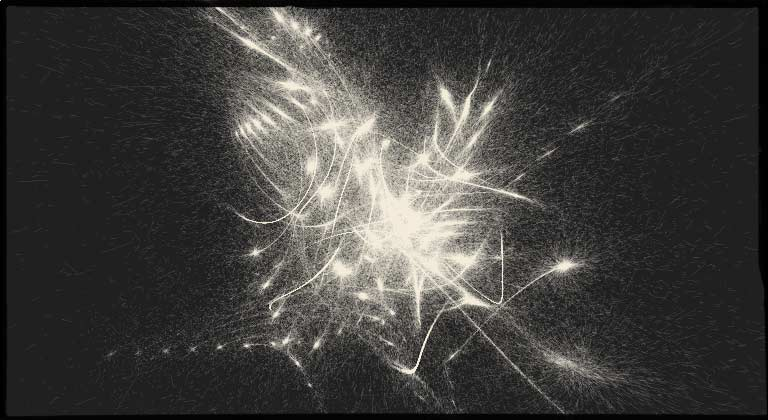
\includegraphics[scale = 0.55]{imgs/ideaspace1.jpg}
\end{center}

\begin{itemize}
\item
Autor: Karsten Schmidt / toxi
\item
Rok: 2004
\item
Médium: generovaná grafika - černobílý tisk
\item
Anotace:
stills of an ongoing visualization project of a space with a steadily increasing number of moving particles attracted by slowly moving, invisible gravitational centres. the cyclic nature of the space itself acts as four dimensional history, causing each particle to leave a persistent trace in time as well as in space. the paradoxical result of this setup is that whereas the number of particles is approaching infinity there's no increase in computational cost.

as the particles move through space they become attracted by the various, initially randomly positioned gravitational centres. the force of attraction follows the classic "inverse square law" in physics, meaning a particle is a lot more influenced and accelerated by a close attractor than by ones further away. the more particles are in a highly active gravitational reqion of the space, the more clearly lines start to appear, showing the trajectory of these particles through space as well as time towards the locally strongest gravitational center.

\end{itemize}

\end{comment}

\chapter{Co je to programovací jazyk?}

\oddil{Jazyk}



\begin{comment}

\pododdil{Definice jazyka}

\begin{enumerate}
\item
K tomu, abychom sdělili informaci, používáme jazyk.


\item
Jazyk musíme umět přizpůsobit tomu, aby informoval, sdělil jistou skutečnost - myšlenku sdělovanému subjektu.

\item
Jazyk má nutně několik úrovní, zdaleka ne všechny jsme schopni reflektovat.

\item
Úrovně, které jsme schopni reflektovat, jen částečně umíme logicky popsat.

\item
Logicky popsaným jazykem a vnitřně uceleným systémem jsme schopni vysvětlit pouhý fragment skutečnosti.

\item
V případě programovacího jazyka si je nutné uvědomit, že programujeme (informujeme) stroj. Dnešní stroje popisují jen zanedbatelně velikou skutečnost fyzicky nepřesahující dimenze součástí stroje\footnote{nejvíce pak procesoru paměti, skutečnost na pevném disku a grafických procesorů}, ale tím zpětně i sebe sama a druhé lidi\footnote{potažmo jakkoli širší skutečnost (zvířata, rostliny, cokoli o čem ani dále netušíme)}, symbolicky a nepřímo popisujeme zkratku skutečnosti nepoměřitelně daleko větší.
\end{enumerate}

\end{comment}

\pododdil{Jednoduchý programovací jazyk}

Snaha po  zpřístupnění programování širší veřejnosti dala již na konci dvacátého století vzniknout rodině jazyků, které jsou patřičně zjednodušeny tak, aby je mohli obsluhovat i neodborníci.

Výchozím bodem pro zjednodušení programování je odpověď na situaci, kdy programovací jazyky vytvářeli především lidé se zvláštním nadáním pro ryze technické uvažování. Technické uvažování je zvláštní nadání, pro které nemá každý člověk správné predispozice. Programování dnes znamená především určitý stupeň svobody při komunikaci se strojem.

K míře svobody, která má své silné kritiky\footnote{včetně mne samotného}, se nyní nechci vyjadřovat, ale zjednodušeně z pohledu pouhého uživatele který používá daný nástroj, schopnost programovat činí z uživatele již potencionálního strůjce vlastních nástrojů.

Hovořím-li o stroji, mám dnes na mysli spotřební počítač. Termín \slovnik{stroj}\index{stroj} používám záměrně pro zdůraznění jisté formy strojového přemýšlení v historickém kontextu.

Nástroje jsou pak programy zkonstruované pro jistou činnost. Obvykle je nástroj vyvíjen za jedním účelem, který plní uživatelsky co nejpřívětivější cestou. Tato cesta je pro uživatele snadno schůdná a nabízí mu standartní škálu dovedností nástroje.

Aniž bychom si to často uvědomovali, současná vizuální kultura je ovlivněna těmito nástroji daleko více, než je na první pohled zřejmé. Technické možnosti jsou současným tržním hladem pro inovaci konfiskovány a proměňovány ve zboží. V této situaci je důležité znát nástroje i jejich vznik pro reflexi nebo kritiku v širších souvislostech.

Tato kniha je spíše než-li jednomu nástroji věnována programu pro tvorbu takových nástrojů. Jak již vyplývá z této definice použití Processingu není limitováno jen úhlem pohledu autora tohoto textu. Návod by se měl stát spíše pobídkou k co nejrozmanitější tvorbě vlastních nástrojů, sloužících opět k co možná nejširší škále možných účelů.

Processing vychází z koncepce snadného přístupu k programování. Za běžných okolností by se vnímavý člověk měl být schopen naučit jednoduché struktuře programu a schopnosti vytvořit vlastní program v průběhu několika dní. Na druhou stranu, právě predispozice našeho uvažování jsou natolik rozmanité, že takovou prognózu nelze brát jinak než-li jen za orientační.


Programovací jazyk processing vychází z laboratoří MIT, kde se celé oddělení věnuje právě koncepcím zjednodušování programovacích jazyků .... historie small talk atd. zde


\pododdil{Dokonalost jazyka}

Co je to dokonalý jazyk? Nejprve je zapotřebí říci, že absolutně dokonalý jazyk neexistuje. Jazyk si můžeme představit jako systém vzájemných vztahů, který je schopen popsat jednotlivé symboly nebo objekty. Symboly můžeme nazvat předměty, tyto předměty dále mají své vlastní hodnoty a vlastnosti, jazyk kromě definic takových vlastností operuje a popisuje jednotlivé jevy a vztahy mezi těmito předměty. Jednodušší popis jazyka je v pojetí výpočetní techniky určitý ucelený systém schopný popsat rozmanité problémy řešitelné strojem.

Co činí předem jakýkoli jazyk absolutně nedokonalým je nejprve fakt, že jakýmkoli jazykem nedokážeme vyjádřit původ jazyka, tj. jeho strůjce; člověka. Jazyk použitý pro instruktáž stroje je vnitřně konzistentní a funguje logicky hermeticky, tj. nepřipouští jiný než jeden výklad konkrétního textu. Pojetí dokonalosti jazyka ve smyslu vnitřní logické konzistence je naprostou nezbytností v pojetí interpretace strojem, na druhou stranu téměř nepřekonatelnou překážkou v případě abstraktnějších úvah o programování jako takovém.

Použiji zde pro názornost rozdíl programovacího jazyka s jazykem českým. Český jazyk, stejně tak jako jakýkoli mluvený nebo psaný jazyk, je jazykem organickým ustáleným po staletí užívání. Jazyk jak ho známe slouží ke komunikaci mezi lidmi, lze tedy použít například pro popis krajiny. Přestože k dokonalému popisu krajiny stěží kdy můžeme dojít, těmito slovy které se opírají o určitou sdílenou zkušenost, lze poměrně dobře přiblížit určitý obraz věcí.

Pokusili bychom se pro popis krajiny použít jazyk programovací, dostaneme se velmi rychle do nesnází. Programovací jazyk není jazykem určeným primárně pro předání informací mezi lidmi, ale pro komunikaci člověka se strojem. Jeho vnitřní logická konzistence, tvrdá logická struktura, která nedovoluje v jeden okamžik jinou než jednu interpretaci, je jeho velikou předností při definici exaktních parametrů. Podobnost s řečí spočívá ve vazbě slov, které reprezentují jednotlivé hodnoty a operace. Hlavní odlišnost je v jeho syntetickém původu, jedná se o jazyk umělý a účelu ke kterému byl zkonstruován. Programovací jazyk je přednostně zkonstruovaný pro definici známého a pochopeného. V případě neznámých nebo nepoznaných veličin, je programovací jazyk víceméně k ničemu. 

Chceme-li komunikovat se strojem musíme tedy svůj způsob vyjadřování přizpůsobit logicky dokonalému jazyku - vnitřní logice fungování stroje. Počítač není navržen k tomu aby něčemu rozuměl, počítač je navržen k řešení jasně definovaných otázek. Tato kniha se pokusí srozumitelnou formou popsat jeden z možných způsobů jak si osvojit takový jazyk a potažmo způsob uvažování, který vede k jasné definici problému. Hovoříme-li o programování, máme na mysli proces tvorby jisté logické struktury. Osvojení si programování spočívá ve schopnosti definovat problém nebo jasně formulovat otázku, tak aby stroj na ni mohl odpovědět.

Vtip celé věci spočívá v tom, že ovládneme-li formálně jazyk určený stroji, můžeme prostřednictvím tohoto stroje hovořit i ke člověku, tj. popisovat pocity z rozkvetlých luk.

\pododdil{Volba jazyka}


Ve výpočetní technice se nachází celá škála programovacích jazyků i prostředí. Tyto jazyky mají svoji genezi a byli historicky vyvíjeny především počítačovými odborníky. Jejich dokonalost lze těžko ocenit z vnějšího pohledu, a to právě z důvodu jejich konstrukce, která odpovídá a částečně podléhá určitým účelům, ke kterým byli tyto jazyky původně navrženy. Celistvý pohled na vývoj programovacích jazyků zde není možné obsáhnout. Základní rozdělení programovacích jazyků dle historického vývoje můžeme dnes označit na dvě skupiny, jazyky procedurální a objektově orientované.

Processing se svojí stavbou na základech Javy řadí k objektově orientovaným jazykům.\footnote{ Jeho společnými příbuznými jsou kromě {\em Javy} jazyky jako {\em C++, C\#,} nebo {\em VisualBasic}} Toto rozdělení pojednává o koncepci jazyka a jeho základních struktur. Ke kterým se dostaneme později. 

V posledních přibližně dvaceti letech se mezi programovacími jazyky postupně objevuje tendence po větší srozumitelnosti a potažmo zjednodušení programování jako takového. Programování v této koncepci zjednodušování již není jen jazykem odborníků, ale je demokraticky přístupný širší veřejnosti z rozmanitých - prioritně netechnických oborů.

Tato tendence postupně dala vzniknout celé rodině programovacích jazyků
\footnote{vyjmenovat jazyky zde + historie?}
které mají ve snaze přiblížit potenciál výpočetní techniky blíže k výtvarné tvorbě. V technických kruzích je již sama disciplína psaní programů považována za tvůrčí. V pojetí výtvarného umění dnes převažuje pohled na programování jako na rigidní a notně limitovanou činnost.

Jazyk, který je nutně limitovaný svojí vnitřní dokonalostí (dokonavostí?) ovšem nemusí nutně limitovat jeho uživatele ve sdělení. Uživatel se ovšem musí do určité míry, naučením se základních struktur, přizpůsobit stroji k uskutečnění zdárné komunikace.

[Důvody pro processing]

\oddil{Tvorba softwaru}

\pododdil{Otevřenost softwaru}

Jazyk nazvaný Processing je jedním z jazyků, který byl vytvořen v diskurzu zjednodušování programování. Jako každý jiný programovací jazyk je i Processing navržen pro jisté účely. V případě tohoto programovacího jazyka se nejvíce jedná o důraz na rychlý vývoj a zjednodušené nakládání s obrazem i prostorem. Z více technického pohledu pak Processing vyniká otevřeností zdrojového kódu a důraz na multiplatformnost.

Z pohledu vývojáře je velmi důležité, že jazyk i programovací prostředí Processing je v současnosti \slovnik{otevřený software}, což znamená, že prostředí i samotný zdrojový kód je volně k dispozici. Processing je dále šiřitelný pod \slovnikpl{MIT licence}. Pro vývojáře otevřenost zdrojového kódu znamená zásadní věc, jednoduše pro dosažitelnost celého zdroje, který se dá následně například implementovat do různých prostředí. Další možnost vývojáře je rozšířit jazyk o vlastní knihovnu, a tím participovat na projektu. Otevřenost kódu teoreticky navyšuje počet možných participantů a de facto celý projekt udržuje v dlouhodobém horizontu naživu.

Z pohledu samotného uživatele je velmi příjemné, že samotný software je k dostání zdarma na stránkách projektu. Za jeho užívání není nutné platit žádné poplatky, a to i v přpadě komerčních užití. V případě potřeby vyjádření vděku za práci autorů je možné zmínit kdekoli ve Vašem produktu \slovnik{Built with Processing}.


Processing na první pohled není ničím zvláštní programovací jazyk. V podstatě by se dalo říci, že se jedná pouze o rozsáhlou knihovnu pro jazyk Java. To co Processing řadí mezi oblíbené softwary pro tvorbu dnes je nejvíce přívětivá komunita uživatelů s velmi odlišnými stupni znalostí a úhly pohledu. Zvláštní důraz je v komunitě kladen na poskytnutí co největší podpory právě začínajícím uživatelům. Tomu odpovídá i počet rozmanitých průvodců a rozsáhlá, velmi dobře stučně napsaná dokumentace ke každému z příkazů v Processingu.

K otevřenosti v kódu v neposlední řadě přistupuje i celá řada velmi zkušených tvůrců. Tím se uživatel na jakémkoli stupni znalostí může kdykoli naučit nové postupy nebo může svobodně recyklovat algoritmy druhých uživatelů. Processing a čím dál více jeho uživatelů ctí filosofii otevřeného softwaru která (mimo jiné) hlásá: \uv{Vědomosti nesmí být privatizovány!}

\pododdil{Procesualita, živý program}

Hlavní doménou Processingu je schopnost vytvářet \uv{živé} programy, tj. programy běžící v reálném čase. Již jméno programovacího jazyka Processing napovídá akcent jisté procesuality, v čase se odvíjející události.

Obraz vytvořený tímto způsobem, na první pohled zaměnitelný s videem, nemusí například podléhat časové omezenosti, nebo může určitým způsobem reagovat na své okolí. Generovaný obraz může být například takto vtažen do kontextu, ve kterém se nachází. Možností jak nakládat s těmito specifickými možnostmi je nepřeberné množství.

[rozvést více]

\pododdil{Empirický přístup k programování}

	I když zásadní odlišnost s jinými programovacími jazyky bychom hledali stěží, Processing proslul zejména pro snadnost použití. Kompilovat program není otázkou nastavování kompileru a veškerých jeho parametrů, program jednoduše po stisku tlačítka {\em RUN} běží (je-li správně napsán). Samozřejmě tento redukcionistický přístup má své nevýhody, speciálně při rozsáhlejších projektech tato jednoduchost může dokonce omezovat. Processing ovšem jako svobodný software lze naimplementovat do řady jiných prostředí, a potřebujete-li si kompilační proces nastavit sami, nic Vám například nebrání použít Processing jen jako knihovnu do {\em Javy}.

Tato základní jednoduchost na druhou stranu nezdržuje uživatele od myšlenkového toku psaní programu. Častou kontrolou výsledku kódu uživatel může lépe interagovat se samotným tvarem programu.

Nazývám tento způsob programování empirický, tedy přístup, kdy podle zkušenosti s běžícím programem je dotvářen i samotný zdrojový kód. Mnoho technicky zaměřených lidí by zřejmě mohlo tento postup kritizovat pro přílišnou reduktivnost a amatérský přístup k programování. Zde bych oponoval faktem, že motivace lidí vytvářející například instalaci do galerie nezajímá příliš dokonalost (když už tedy vůbec) programu. Program je v pojetí tvůrců jen prostředníkem pro další sdělení, a jestliže toto sdělení předá je to dobrý program.

Proces poznávání struktur jazyka při tvorbě obrazu prostřednictvím Processingu bych přirovnal k postupu od začátečnické malby na tkaninu k postupnému tkání gobelínu. Zde je nutno podotknout, že ne každý tvůrce využívající Processing chce tkát gobelín a najde-li nástroj vhodný \uv{jen} pro \uv{malbu} na plátno, je to dobrý nástroj.


[????]

\chapter{Processing jako prostředí}


Processing představuje ucelené programovací prostředí tzv. IDE\footnote{Integrated Development Enviroment}. Jedná se o kompletní prostředí určené především k rychlému vývoji aplikací. Samotný program je jednak otevřeným softwarem\footnote{tj. s otevřeným veřejně dostupným zdrojovým kódem}, a také zdarma ke stažení pro všechny majoritní platformy. Processing je k dispozici pro \slovnik{GNU / Linux}, Mac OS i pro Microsoft Windows na stránkách projektu processing.org. Porcessing je teoreticky možné spustit v jakémkoli prostředí umožňujícím chod Javy. Celý jazyk i samotné IDE vychází pod licencí \slovnik{GNU / GPL} jedná se tedy o svobodný software. Díky této licenci můžete jakýkoli výstup z tohoto softwaru můžete publikovat, použit pro jakékoli účely včetně například užití v komerčních aplikacích.


\pododdil{Sketch}

Sketch, neboli náčrt, označuje samostatný projekt Processingu. Dělením projektů na sketche jsou uspořádány jednotlivé projekty Processingu. Sketch je ve své podstatě složka obsahující alespoň stejně jeden stejně nazvaný soubor s příponou {\em *.pde}. Sktech při vytvoření nevyžaduje název, je jí přidělen pouze aktuální datový kód zaznamenávající datum vytvoření. Tímto decentním způsobem Processing toleruje například nejasnost záměru autora při vytváření nového díla, jeho název či pracovní název lze tímto způsobem přiřadit až později, po nabytí jasnějších obrysů.

Program si vystačí pouze se samotným zdrojovým kódem tj. souborem (soubory) {\em *.pde}. Ovšem v případě operujeme-li s externími daty stojícími mimo zdrojový kód, jakékoli jiné soubory, můžeme využít dvě možnosti. První možnost je soubor, se kterým potřebujeme operovat tažením myši přesunout na textové pole Processing \index{IDE}IDE. Touto operací bude soubor zapsán do naší sketche automaticky. Druhá možnost je operaci provést manuálně, stačí vytvořit v adresáři sketche adresář s názvem \slovnik{DATA}. Processing tuto složku automaticky rozpozná a soubory v této složce budou dobře dostupné pro pozdější operace.

Ke standartním adresářům, které se často objevují ve struktuře skteche, si stačí zapamatovat jen dva již zmíněný adresář nazvaný {\em DATA}. Tento adresář je využíván při práci s jakýmikoliv vnějšími daty jako jsou např. obrázky, zvuky, videa, vektorové grafiky nebo například textové soubory. Druhý adresář nazvaný {\em CODE} obsahuje externí zdrojový kód, popřípadě kód kompilovaný v podobě knihovny, mající nejčastěji přípony {\em *.java, *.class, *.jre}. Tento adresář se nalézá v systémové cestě daného projektu a umístíme-li zde soubory budou též dobře dostupné z daného projektu. Adresář {\em CODE} nás zatím nemusí příliš zajímat, později se jeho prostřednictvím můžeme pokusit rozšiřovat funkce Processingu.


\pododdil{Sktechbook a uspořádání}

Místo na disku, které Processing využívá k uskladnění sktechí se nazývá povšechně sketchbook a je v podstatě pouze adresář obsahující jednotlivé projekty. Koncepce sketchbooku spočívá v uspořádání jednotlivých projektů do organizované formy a ačkoli nevnáší do jednotlivých projektů sám o sobě řád může napomoci k vytvoření řádu vlastního. Ze své zkušenosti mohu říci, že organizace jednotlivých projektů do jakékoli struktury má opravdu smysl. Mnou preferovaná struktura obsahuje jednotlivé roky následně ještě dělené do měsíců, ale možnosti organizace záleží čistě na uživatelových preferencích. Tímto chci spíše ilustrovat možnosti uspořádání než-li nezbytnost, ale přítomnost vašeho systému od počátku vřele doporučuji.

Ve sketchbooku se dále nachází jeden speciální adresář nazvaný {\em libraries}. Adresář v sobě uchovává externí rozšíření Processingu o komunitní knihovny. Standartně Processing již své základní knihovny nese v sobě, tj. jsou standartně přidány do samotného Processingu. V tomto adresáři se nacházejí knihovny které budete moci použít později. Na stránkách projektu {\em http://processing.org} můžete nalézt velké množství komunitních knihoven s dobrou dokumentací, volně ke stažení. Veškeré tyto knihovny tedy Processing potřebuje nalézt v tomto adresáři.


\oddil{Základní prostředí}


Základní rozhraní tvoří textový editor s několika nezbytnými funkcemi. Patrně nejdůležitější je v liště tlačítko (1) tzv. RUN. Které kompiluje a spouští program aktuálně rozpracovaný v textovém editoru. (2) Tlačítko STOP naopak program zastaví. V případě chyby v programu lze též využít jako vynucené zavření programu. Zbylé tlačítka slouží k diskovým operacím. \\


\begin{center}
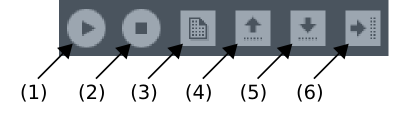
\includegraphics[scale = 1]{imgs/buttons.png}
\end{center}


\newpage
\pododdil{Základní diskové operace}

Ty operace jež něco zapisují či načítají z disku. Tyto opera zahrnují veškerou manipulaci se sketchí, její vytvoření, uložení, načtení či export do webového formátu či kompilaci do spustitelné aplikace.

Processingová sketch nemusí být nutně uložena aby jste ji mohli spustit. Nové úpravy, které v textovém poli napíšete budou dočasně uloženy v závislosti na vašem operačním systému jinde. Tímto způsobem můžete experimentovat s kódem aniž by jste přišli o předchozí verzi.

Mezi základní operace patří vytvoření nové sketche (3), otevření předešlé (4), uložení (5) a export (6).

Tlačítka mají dále speciální vlastnosti s podržením tlačítka tlačítko s novou sketchí otevře také nové okno editoru. V kombinaci s načtením předchozí sketche (4) otevřete též sketch v novém editoru aniž by jste ztratili předchozí okno. U uložení se modifikace projevuje funkcí uložit jako. U exportu stisknutím klávesy \klavesy{SHIFT} přepínáte mezi exportem samostatné aplikace nebo tzv. appletu, aplikace schopné běžet v prohlížeči nebo obecně na webových stránkách.

\pododdil{Editor}

Editor je textové pole a je vaším hlavním komunikačním nástrojem s Processingem. Veškeré informace které zadáte do tohoto pole budou interpretovány samotným Processingem. Textový editor není nijak dokonalý, pro začátek si s ním ovšem vystačíme. Formát který tento editor produkuje je ve své podstatě textový soubor s příponou {\em *.pde}.




Textový editor má několik funkcí, které vám mohou usnadnit práci. Odlišuje například mezi příkazy Processingu odlišnými barvami, tato zdánlivá banalita vám speciálně v začátcích nebo v případě objemnějších kódů může výrazně zpřehlednit organizaci programu. Jedná se o programátorskou konvenci obecně v anglickém jazyce nazývanou \slovnik{syntax highlighting}.


Další konvencí se kterou se často setkáte je tzv. \slovnik{indenting}, zarovnávání kódu do úhledných paragrafů. V Processingu si ze začátku vystačíte se standartím zarovnáním, posléze lze zarovnávání aktivovat stiskem kombinace kláves \klavesy{CONTROL (APPLE) + T}.

Více o konvencích se dočtete na straně~\pageref{Předmluva}

\begin{center}
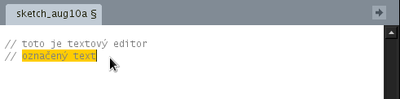
\includegraphics[scale = 0.75]{imgs/editor.png}
\end{center}

Horní lišta editoru označuje záložky, kliknutím na šipku v na pravé straně lišty se vám zobrazí možnosti operací se záložkami. Pro začátek s nimi nebudeme operovat. V případě delšího kódu záložky slouží k lepší organizaci struktury programu. V podstatě se dá říci, že každá záložka odpovídá jednomu souboru ve sketchi. Co je to sketch popíšu níže.

Jak můžete vidět na obrázku editor operuje i českými znaky, ačkoli bych jejich používání z důvodů internacionalizace neradil používat. V komentářích tj. textem uvozeným dvěma dopřednými lomítky {\em //}, tedy text, který kompiler ignoruje, jsou diakritická znaménka přípustná.

Naopak v případě názvu proměnných, nebo jakýchkoli funkčních definic, je použití diakritiky v devadesáti procesntech nefunkční.\footnote{standartní jazykové kódování, ve kterém Processing operuje je {\em UTF-8}}




\chapter{Processing jako jazyk}



\oddil{Syntax}

\oddil{Základní pravidla a zvyklosti}

V programování obecně platí jisté zákonitosti. Není tomu jinak i u pravidel, které nejsou důležité pro čtení kódu strojem ale pro člověka. Speciální zákonitosti formátování kódu mají ryze praktickou funkci. Jedná se o standart dodržovaný programátory, tak aby mezi sebou byli schopni sdílet své úsilí.

\index{flow}

V problematice programování obecně platí, že není nic složitějšího, než číst cizí kód, nebo dokonce vlastní s odstupem času. Při programování se lidská mysl dostává do stavu mimořádné bdělosti tzv. \slovnik{flow}\index{flow}, stavu ve kterém mysl vědomě drží celý\footnote{nebo větší části} programu.

Pokaždé když si programátor navodí takový stav, vše v kódu\footnote{podle míry ovládnutí programovacího jazyka} se pro něj jeví srozumitelné. Formátování a standarty velmi napomáhají k rychlému navození bdělého stavu, protože sami o sobě jsou jistou formou jazyka.


\oddil{Orientace v prostoru}

Plocha programu by sa dala přirovnat k listu papíru, popřípadě k malířskému plátnu. Ve standartním dvoudimenzionálním módu má dva základní parametry {\em X} a {\em Y}, ty označují souřadnice, ve kterých se veškeré kreslící operace pohybují. Důležité je zmínit, že oproti jisté konvenci v matematických grafech levý horní roh nese hodnotu {\em X = 0}, {\em Y = 0}. Směrem dolů hodnota {\em Y} přibývá stejně tak jaho hodnota {\em X} přibývá směrem doprava.\\

\begin{center}
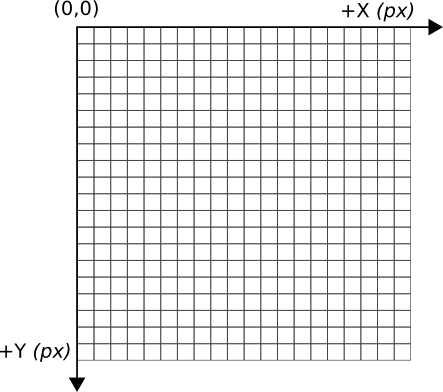
\includegraphics[scale = 1]{imgs/grid2d.png}
\end{center}

Tato konvence je převzata ze standartu počítačové grafiky, kdy první pixel v levém horním rohu nese souřadnicovou hodnotu právě {\em X = 0}, {\em Y = 0}. Obrácená osa Y se může ze začátku jevit matoucí. Důvody pro zdánlivé převrácení os pochopíme později například právě při operacích se samotnými obrazovými body, pixely, které jsou standartně uspořádány od levého horního rohu doprava a níže.

Plochu je možné představit si jako prázdný prostor, na kterém je možno zobrazovat grafiku. Tvary nebo například text se zobrazují právě prostřednictvím zdrojového kódu tj. instrukcemi psanými v editoru.

Na první pohled by se mohlo zdát, že například při zobrazení obdélníku, příkaz:

\begin{lstlisting}
rect(x,y,šířka,výska);
\end{lstlisting}

jehož výsledkem je kresba pouhého obdélníku je zbytečně komplikovaný, oproti jiným zobrazovacím metodám. Důležité je si zde uvědomit koncepci Processingu, který tímto zobrazením primitivních objektů sestavuje celý obraz. To co se zpočátku může zdát jako nadbytečná práce, tj. psaním koordinátů každého ze zobrazovaných objektů se posléze ukáže jako sofistikovaný a velmi ulehčující způsob přemýšlení o obraze. Veškeré parametry oddělené čárkou v kulatých závorkách příkazu {\em rect} náleží samotným vstupním hodnotám. Příkaz {\em rect} očekává čtyři parametry. Parametry mohou být celá čísla nebo čísla s desetinnou čárkou. Pro názornost, zadáme-li do parametrů ''natvrdo'' hodnoty:

\begin{lstlisting}
rect(8,6,7,5);
\end{lstlisting}

Výsledné zobrazení na naší pomyslné ploše bude následující:

\begin{center}
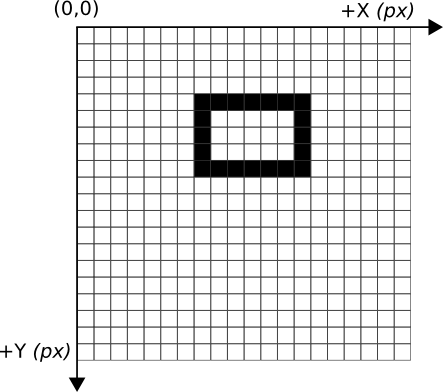
\includegraphics[scale = 1]{imgs/gridRect2d.png}
\end{center}


Zamyslíme-li se například o tom, že bychom v jakémkoli jiném nástroji chtěli zobrazit vícero, například tisíc obdélníků, na první pohled jednodušší GUI \footnote{zkratka pro "Guided User Interface" klasické grafické editory jako Gimp nebo Photoshop} grafické editory nám nedovolí tuto operaci učinit jinak, než že musíme všech tisíc obdélníků nakreslit. V případě Processingu nám bude stačit vytvořit rutinu pro kreslení libovolného počtu obdélníků a pak tuto rutinu spustit.

Zde se již dostáváme k samotnému jádru Processingového přemýšlení. Programování obecně dokáže velmi ulehčit operace jejichž pravidelnost dokážeme popsat. Veškeré umění psaní programu tedy spočívá v definicích těchto chování a redukci složitých jevů na jednoduché rovnice.

Celé řemeslné umění psaní kódu v podstatě záleží na eleganci v zápisu složitějších vztahů mezi různými parametry. Dovednosti se člověk učí postupně, osvojení si gramatické korektnosti a logické posloupnosti se mohou zpočátku jevit zbytečně komplikované, ovšem i po ovládnutí pouhých pár jednoduchých pravidel lze Processing využít kreativním způsobem.

V další části se budeme zabývat stavbou programu. Pod odpudivým názvem se skrývají právě tato jednoduchá pravidla, která by měla tvořit základ dalším experimentům.   

\newpage
\oddil{Stavba programu}

\pododdil{Logika programování}
Pro začátek je dobré si představit program jako sadu instrukcí. Každá instrukce má svůj význam a své místo. Instrukce se píší v programovacím jazyku a jejich interpretace je vždy pro stroj jednoznačná. Stroje podle svého návrhu nedělají nic kromě toho co mají takovým způsobem instruováno.

Veškeré programy které používáte, dokonce i programy, které nevíte že používáte byly někdy naprogramovány lidmi pomocí programovacích jazyků. Programovací jazyk je pouze, plánovací forma zápisu programu. K tomu, aby byl program spuštěn, musí být v případě jazyku Processing převeden do strojového kódu. Strojový kód se liší od toho zdrojového, našeho čitelného plánovacího jazyka, tím že není čitelný pro člověka, je čitelný pro stroj.

Počítač je "rychlý blbec". Umí rychle vykonávat sled banálních operací. Programovací jazyk slouží k vytvoření smyslu ve sledu banálních operací. Procesu převodu ze zdrojového kódu do strojového se nazývá kompilace.

O kompilaci toho nemusíme naštěstí vědět mnoho, vše bylo již tvůrci Processingu shrnuto pod tlačítko spustit.

\pododdil{Základní datatypy}

Ke stavbě programu potřebujeme stavební materiál. Pro základní pochopení fungování programu je nezbytné nejdříve pochopit základní datatypy. Datatyp si lze obecně představit jako obálku na informaci.

Processing rozlišuje mezi jednotlivými datatypy. Informace, které se nacházejí v paměti se musí nacházet pod správným datatypem, tak aby program věděl jak s nimi operovat.

Pro datatyp je možné představit si různé paralely, má oblíbená je podobnost s obálkami nebo nádobami. Různé datatypy si můžeme představit jako tvary nádob. Do různých nádob, lišících se tvarem, se směstná různý obsah. Typy obsahů se dají názorně představit na rozdílu mezi textovou informací a informací číselnou.

Processing potřebuje nejdříve vědět zda nádoba obsahuje text nebo číslo, aby mohl s touto nádobou operovat. Například, nelze provést matematickou operaci mezi dvěma slovy. Sčítat, odčítat, dělit či násobit se dají pouze čísla.


\pododdil{Seznam základních datatypů}
Datatypů je jen několik, dají se vcelku snadno zapamatovat:

\begin{lstlisting}
int mojeCeleCislo = 1;

float mojeCisloSDesetinnouCarkou = 1.33;

boolean mojePravdaCiNepravda = true;

String mujSlovniRetezec = "Ahoj svete!";

char mujJednotlivyZnak = 'A';

color mojeBarva = color(255,127,1);
\end{lstlisting}

Takovému zápisu bude již Processing rozumět. Vepsáním těchto řádků do processingového editoru již dochází k alokaci vašich informací ve správných datatypech v paměti. Vysvětleme si nyní několik nejasností.

První slovo na každém řádku označuje odlišný datatyp (náš tvar nádoby), následuje jméno proměnné (název pro naší nádobu), poté následuje rovnítko které již přiřazuje obsah - hodnotu do proměnné (nádoba je naplněna).

Každý příkaz je ukončen středníkem {\em ;} .

Podivné názvy jako například {\em mojeCeleCislo} tzv. proměnných, jen ukazují, že název pro svoji proměnnou můžete zvolit téměř podle libosti. Co do výjimek v názvech proměnných. Proměnná nesmí mít v názvu mezeru tedy prázdný znak. Podle zvyklostí by dále proměnná měla začínat malým písmenem a potřebujete-li nutně pro název použít víceslovný název použijte velké písmeno namísto mezery.

Proměnná nesmí být číslo, ale slovní název. Programátorské konvence při pojmenovávání proměnných jsou ryze praktické. Proměnná by měla mít co možná nejkratší a nejvýstižnější název.  Toto je spíše dobré doporučení než-li pravidlo. Správným pojmenováním proměnných docílíte větší přehlednosti v kódu kratší délkou si ušetříte zbytečné psaní.

\pododdil{Tisk do konzole}

Tento jednoduchý program, zatím jen definoval pár proměnných do správných datových typů zatím nedělá nic zajímavého. Celá alokace probíhá uvnitř programu. Processing dělá většinu svých operací skrytě. Program kreslí nebo jinak interaguje s uživatelem jen je-li o to požádán.

Nejjednodušší výstup z programu je tisk do tzv. konzole. Konzoli jsme si již krátce uvedli v kapitole {\em Základní prostředí}. V Processingu se konzole nachází pod textovým editorem. Toto černé pole má pouze textový výstup a slouží k odladění programu.

Tiskem do konzole si nyní můžeme například zkontrolovat obsah našich proměnných. To můžeme provést následujícími dvěma způsoby:


\begin{lstlisting}
print(mojeCeleCislo);

println(mujSlovniRetezec);
\end{lstlisting}

Oba příkazy tisknou obsah našich proměnných. Jediný rozdíl mezi příkazy je ten, že druhý příkaz končí znakem:
 
\begin{lstlisting}
"\n"
\end{lstlisting}

jedná se o tzv. {\em newline character}, přidáním speciálního charakteru příkaz tiskne pokaždé na nový řádek. Není nutné si pamatovat tento speciální znak, postačí když si zapamatujeme příkaz {\em println( cokoli );}

Spustíme-li program nyní, v konzoli se nám ukáže výstup z našeho programu:

\begin{lstlisting}
1ahoj světe!
\end{lstlisting}

Zde je názorně vidět, že tisk pomocí pouhého příkazu {\em print} nepoložil další příkaz na nový řádek, a tedy vytiskl {\em 1ahoj} dohromady.

Tisk do konzole se hojně používá při ladění programu. Kdykoli se na něco potřebujete kódu zeptat můžete tak učinit tímto prostým příkazem.

V konzoli se tisk projevuje bílou barvou. Další možný obsah konzole jsou chyby. Ty jsou označeny barvou červenou. Processing vám chybou naznačuje, že něco není v pořádku s vaším kódem. V případě takto jednoduchého programu se v drtivé většině případů bude jednat o překlep, či zapomenutý znak.

Programovací jazyk bohužel (naštěstí ?) neodpouští žádné překlepy. Tedy bude stačit jeden chybný znak v programu aby celý program nebyl spustitelný.

Bohužel chybové hlášení se nedá označit za dokonalé a pro začátečníky bude velmi složité dobrat se pomocí chybových hlášení k původu chyby. Na zlepšení chybových hlášek se pracuje již dlouhou dobu a některé základní chyby Processing v angličtině umí dobře popsat. Většinou ale Processing tiskne řetězec svých chyb, které byly nastartovány chybou vaší a chybová hlášení čítající několik desítek řádků vám toho nakonec o původní chybě moc nesdělí.

V případě chyby se vás Processing bude snažit přesměrovat na řádek, kde chyba pravděpodobně vznikla. V případě takto jednoduchých programů, jaké si zde ukazujeme, chybu identifikuje zcela bezchybně, bohužel tomu tak nebude ve všech případech.


\pododdil{Základní operace s datatypy}

Náš program nyní nedělá nic světoborného. Definuje pár proměnných a následně některé z nich tiskne do konzole. Operujeme zde stále s abstraktními hodnotami které se zapisují do paměti programu a ty pak z paměti zpětně získáváme.

Nyní si ukážeme co s již definovanými proměnnými můžeme dělat. Jednotlivé datatypy mají různé přípustné operace. Zkusme si letmo projít možnosti našich proměnných.

\begin{itemize}


\item{Integer a Float, neboli čísla: {\em int a float}}

První proměnná {\em mojeCeleCislo}, které byla přiřazena hodnota {\em 1}, je takzvaný {\em Integer}, tedy celé číslo. Tento typ může mít hodnotu\footnote{na 32-bitových strojích} v rozsahu {\em -65575 až 65576} [upřesnit] . V rozmezí těchto hodnot můžeme provádět různé matematické operace mezi čísly:

\begin{lstlisting}
int prvniCislo = 1;
int druheCislo = 5;
int tretiCislo;

tretiCislo = prvniCislo + druheCislo;

println(tretiCislo);
\end{lstlisting}

Tímto jsme provedli základní matematickou operaci, sečetli jsme dvě čísla a následně jsme výsledek vytiskli do konzole.

Další možné operace jsou:

\begin{lstlisting}
// aritmetické operace
a + b;
a - b;
a * b;
a / b;

// přírůstky
a += b;
a -= b;

// přírůstek, úbytek o 1
a ++;
a --;

// modulo (přebytek po dělení)
a % b;

// a konečně logické porovnávání
// větší, menší
a < b;
a > b;

//větší nebo rovná se, menší nebo rovno
a <= b;
a >= b;

// shoda, neshoda
a == b;
a != b;

// pozor výsledkem porovnávání již není číslo!
// ale odpověď ANO nebo NE, TRUE nebo FALSE
// pravda nebo nepravda, datatyp boolean

\end{lstlisting}

Celá čísla neboli {\em int} nebudou mít problém se sčítáním, odčítáním a násobením celých čísel. V případě dělení může nastat logicky problém, výsledek nemusí být celé číslo. Budeme-li chtít výsledek takové operace uchovat v paměti, tj. zapsat pod naši proměnnou, musíme použít datatyp operující s desetinou čárkou, nebo výsledek zaokrouhlit na celé číslo.

například:

\begin{lstlisting}
int a = 10;
int b = 3;
float c;

c = a / b;

println(c); 
\end{lstlisting}

Vytiskne {\em 3.0}. Pozor, to není správný výsledek! Kde se stala chyba? Processing operující s celými čísly, speciálně při dělení předpokládá výsledek opět za celé číslo. Tedy ono zaokrouhlení provádí již sám. Zde si dovolím nesouhlasit s tvůrci, kteří se tímto snaží začátečníky vyvarovat chyb. Stačí si nyní pamatovat, že pro přesné dělení čísel bychom měli dělit vždy číslem s desetinnou čárkou, tj. s datatypem {\em float}.

Tedy správně by dělení mělo proběhnout takto:

\begin{lstlisting}
float a = 10;
float b = 3;
float c;

c = a / b;

println(c); 
\end{lstlisting}

Tisk do konzole již ukazuje správnou hodnotu {\em 3.333333} .

Pro další operace s čísly bych pro přesnost výsledků důrazně doporučil používat jen float. Další operace mohou vypadat například takto:

\begin{lstlisting}
float a = 3;
float b;

// sq je funkce pro "square", číslo na druhou
b = sq(a);
println(b);

// sqrt je funkce pro "square root", odmocninu
b = sqrt(a);
println(b);

// pow je funkce pro "power", číslo na N-tou
// mínusová čísla v N jsou odmocniny
b = pow(a,3);
println(b);

b = pow(a,-3);
println(b);

// atp.
\end{lstlisting}

\item{{\em char a String}, znak a řetězec znaků, text}

S textem nelze operovat stejně jako s čísly, je logické, že nemůžeme násobit texty mezi sebou. {\em String} je speciální datatyp pro uchovávání textů v paměti a nakládá se s ním speciálními funkcemi. Prozatím nám bude stačit, když si ukážeme velmi jednoduchou operaci s textem, spojení dvou řetězců dohromady.

Pro označení hodnoty řetězce se používají dvojité uvozovky. S textem se pracuje následovně:

\begin{lstlisting}
String prvniSlovo = "Ahoj";
String druheSlovo = "světe!";
String slovniSpojeni;

slovniSpojeni = prvniSlovo + " " + druheSlovo;

println("Dvě spojená slova: " + sovniSpojeni);
\end{lstlisting}

Všimněte si prosím vloženeé mezery mezi slova " ". Uvozená mezera je počítána také jako řetězec textu. Výsledným tiskem do konzole tedy dostaneme následující řetězec textu:

\begin{lstlisting}
Dvě spojená slova: Ahoj světe!
\end{lstlisting}

Zde jsme provedli jednu ze základních operací s textem, spojování řetězců. {\em String} lze také spojit s jednotlivými znaky, nebo také s čísly, výsledkem bude ovšem vždy další {\em String}.

\begin{lstlisting}
int a = 1;
int b = 2;
String slova = "test";

// "slova = slova + něco" lze také nahradit znaménkem "+="
// stejným znaménkem které u čísel znamená přírůstek
// tedy namísto:
// slova = slova + " " + a + " " + b;
// můžeme zkrátit na:

slova += " " + a + " " + b;

println(slova);
\end{lstlisting}

Výsledkem bude: {\em test 1 2}.

Řetězce se dají dále porovnávat seřazovat, dá se v nich vyhledávat znak či slovo a tak podobně. Pro náše účely zatím postačí si uvědomit rozdílné operace mezi textem a číslem.


\item{{\em boolean}, neboli pravda nebo nepravda}

Boolean je nejjednodušším datatypem v Processingu, může vyjadřovat pouze dva stavy. Pravdu {\em true}, nebo nepravdu {\em false}. Žádnou jinou hodnotu {\em boolean} nepřijímá a je proto  ,co se paměti týče, velmi úsporný datatyp. Operace s booleany se nazývají logické operace a vypadají následovně:


\begin{lstlisting}
boolean prvniTvrzeni = true;
boolean druheTvrzeni = false;
boolean tretiTvrzeni;

// "&&" značí logickou operaci AND
// výsledek bude TRUE, pravda, JEN pokud
// prvniTvrzeni a druheTvrzeni bude pravda
tretiTvrzeni = prvniTvrzeni && druheTvrzeni;

println(tretiTvrzeni);

// "||" dvě svislé čáry je OR, tj "nebo"
// výsledek bude TRUE, pravda pokud
// prvniTvrzeni nebo druheTvrzeni je pravda
tretiTvrzeni = prvniTvrzeni || druheTvrzeni;

println(tretiTvrzeni);

// posledni zakladni operaci je porovnani
// muzeme porovnat dva booleany pomoci "=="
// dvojiteho rovnitka
tretiTvrzeni = (prvniTvrzeni == druheTvrzeni);

println(tretiTvrzeni);

// pro negativni vysledek je zaporne porovnani "!="
// vykricnik pred booleanem vzdy znaci opak

tretiTvrzeni = (prvniTvrzeni != druheTvrzeni);

println(tretiTvrzeni);

\end{lstlisting}

Boolean je možné si představit jako vypínač světla. Zapnuto a vypnuto jsou jediné dva stavy podobného vypínače. Booleany často řídí tok programu, je možné si je představit jako přepínače mezi jednotlivými stavy programu.

\end{itemize}

\pododdil{Podmínka}

Uvedením do stavů programu se můžeme dostat k první opravdové struktuře v programu. Zkusme nyní nastínit jak taková struktura vypadá. Patrně nejpřímější řízení dějů v programu je podmínka. Podmínka říká, jestliže je něco pravda, spusť následné příkazy. Uvedu zde krátký příklad podobné struktury:

\begin{lstlisting}
boolean prepinac = false;
int hodnota;

if(prepinac == true){
    hodnota = 1;
}else{
    hodnota = 0;
}

println(hodnota);

\end{lstlisting}

Velmi prostá struktura je v tomto příkladě vytvořená jednou podmínkou. Podmínka je v Processingu (a řadě jiných jazyků) značena slovem {\em if}, "jestli". "Jestli" potřebuje dostat odpověd v kulatých závorkách, ta může být jen pravda nebo nepravda, k tomu se hodí nejlépe již zmíněný {\em boolean}, nebo například porovnávání dvou čísel, znaků nebo řetězců znaků, tj. operace které nám vrátí {\em TRUE} nebo {\em FALSE}.

Definujeme-li tedy náš {\em boolean} na začátku jako nepravdu, podmínka se v tomto případě nenaplní a program spustí kód uvozený složenými závorkami následujícími až slovo {\em else}.
V našem příkladě se jedná o druhou větev podmínky, ta sice není povinná ale pro ukázku jsem ji zde rovnou zmínil. Tedy za ukončením {\em if} a složených závorek můžeme dále slovem {\em else}, tzn. "jestliže ne", řící co se stane v případě nenaplnění naší podmínky.

V tomto konkrétním případě se k proměnné {\em hodnota} přiřadí číslo {\em 0}.

To program následně ověřuje tiskem do konzole, kde se objeví {\em 0}.

\oddil{Hodnota a její zobrazení}

K čemu jsou vlastně hodnoty dobré? Tisk do konzole je jen kontrolní mechanismus většinou se nejedná o výslednou podobu programu.

Po celou dobu sčítání a odčítání hodnot jsme nezavolali žádnou funkci, která by kreslila na plátno.

Nyní je na čase ukázat si jakým způsobem Processing rozumí kresbě. Ty samé hodnoty které máme nyní v paměti mohou být použity pro jakýkoli kreslící výstup. Řekněme že chceme z těchto hodnot zobrazit například elipsu. K tomu potřebujeme zavolat funkci pro tvorbu elipsy, pokud ji nechceme zrovna z nějakých důvodů popisovat matematicky (to je samozřejmě dokonale možné).

Processing nemá předdefinované žádné složité tvary. Pracuje sám o sobě pouze s tvary primitivními, jako je bod, linka, trojúhelník, obdélník a elipsa. Pomocí těchto tvarů lze zkonstruovat nepřeberné množství obrazů. Představíme-li si nyní digitálně zpracovanou fotografii, můžeme například říci že je zkonstruována z bodů. Jednotlivé body, tj. pixely mají jinou barevnou hodnotu a takto poskládaný obraz se ve výsledku jeví jako fotografie.

Problém v případě konstrukce syntetické fotografie nespočívá v geometrii; ta je známa, mřížka bodů s počtem šířky krát výšky obrazových bodů digitální fotografie. Problém je v barevných hodnotách, které neznáme a synteticky jakoukoli matematickou funkcí těžko obsáhneme.

Tento příklad je trochu extrémní, ale naprosto pravdivý. Věc kterou se snažím ilustrovat je ta, že i s minimálním počtem primitivních geometrických tvarů lze docílit téměř nekonečné (spočitatelně obrovské) množství obrazů, což by nám mělo nadlouho stačit.

Nyní zpět k hodnotám. Máme-li již jakékoli hodnoty v paměti programu, můžeme kterékoli z nich namapovat na jakoukoli kreslící funkci. Zde začíná naše experimentální část, často se totiž stává, že výsledek kreslení neumíme plně předpovědět a teprve zobrazením nám kresba vzhledem k hodnotě začne dávat smysl.

Processing je, co se týče grafického výstupu, navržen pro přímou experimentální interakci vznikajícího programu s uživatelem. To znamená, že pokaždé kdy chcete vidět výsledek kódu, stačí pouze stisknout tlačítko {\em RUN}. Zpětná vazba spolu s vaší interpretací a úmyslem má potom veliký vliv na následné úpravy v kódu. Tímto způsobem můžete doslova "vysochat" výslednou podobu programu.

\pododdil{Zobrazení}

Jak zobrazit hodnoty, které uchovává program v paměti? Jakákoli hodnota lze použít například jako jeden z argumentů v kreslících funkcích.

Již zmiňovaný {\em rect}, tedy rectangle - obdélník, vyžaduje ke svému úspěšnému vykreslení čtyři parametry, čtyři číselné hodnoty \footnote{zde nezáleží jestli se jedná o celé číslo int nebo číslo s desetinnou čárkou float}. Tyto parametry, hodnoty, můžeme buďto zadat jako přímé číselné hodnoty, nebo do těchto parametrů můžeme zadat naši proměnnou která obsahuje číslo. Názorně:

\begin{lstlisting}

// první způsob vykreslení obdéníku
rect( 10, 8, 40, 20 );

// druhý způsob vykreslení obdélníku
int prvniCislo = 10;
int druheCislo = 8;

rect( prvniCislo, druheCislo, 40, 20 );

\end{lstlisting}

Již nyní je nám zřejmé jak hodnoty mohou ovlivnit zobrazení. Namísto hodnot zadaných číselně se zde v druhém způsobu vykreslení obdélníku objevují naše proměnné, které mají již zadaný obsah. Výsledek zobrazení bude v obou případech stejný, ovšem z hlediska struktury programu je druhý způsob daleko flexibilnější.

Představme si nyní, že hodnota zadaná prvním způsobem zápisu se již nikdy v průběhu programu nemůže proměnit. V případě druhého způsobu zápisu získáváme díky možnosti změny jednoho parametru kontrolu nad kreslícím výstupem.

Veškeré příkazy které jsme si zatím ukázali byli spuštěny pouze jednou. To znamená, že obdélník byl vykreslen a program, který již neměl žádné další příkazy jednoduše skončil.

V další kapitole si předvedeme jak vdechnout procesům pohyb a stálost, další kapitola je věnovaná animaci.

\oddil{Animace a interakce}
\index{animace}

\pododdil{Animace}

Statická kresba na plátno je jen jeden z možných výstupů. Animace v Processingu znamená překreslovat plátno pokaždé jinými obrazy. Processing je jazyk využívaný zjeména v pohyblivém obraze. Nyní si ukážeme základní postup při tvorbě pohyblivého obrazu.

Základní funkce pro vyvolání překreslování výstupního okna je funkce \vyraz{draw()}. \bublina{void draw() je základní funkce pro spuštění překreslování plátna} Funkce je uvozena slovem \vyraz{void}. Více o funkcích se dozvíme v kapitole. Jedná se o základní smyčku, která zajišťuje jakoukoli proměnlivost, tedy animaci v obraze. Smyčka je de facto operace, která v programu vyjadřuje rozměr času.

Velmi zjedoušeně řečeno smyčka je prostředek pro změnu není změnou sama o sobě. Smyčka zajišťuje sousledné volání příkazů v neustálém trvání\footnote{po dobu běhu programu}. V Processingu si v podstatě uvědomíme, že psaním příkazů do smyčky píšeme pravidla jakoby pro jedno okénko ve filmu. Pohyb je vždy zajištěn proměnou našich datatypů, které v tomto okénku figurují.

Tedy například napíšeme-li takto, samotnou smyčku:

\begin{lstlisting}
void draw(){
	// 60x za vteřinu spuštěná operace
}
\end{lstlisting}

Vše uzavřeno do složených závorek bude spuštěno šedesátkrát za vteřinu. Bude-li obsah základní funkce \vyraz{draw()} neměnný, tj. budeme-li volat šedesátkrát za vteřinu to samé, animace bude ovšem jen abstraktní pojem.

V tomto příkladě již dochází ke spuštění smyčky. Výsledkem bude pouze šedivá plocha v rozměrech sto krát sto pixelů, jelikož na plátno nebylo zatím nic vykresleno. Následujícími příkazy \vyraz{background()} a \vyraz{rect()} nakreslíme nejprve plné pozadí a následovně obdélník. Zápis bude vypadat následovně:

\begin{lstlisting}
void draw(){
	// pozadí
	background(255);
	// obdélník se čtyřmi parametry
	rect( 10 , 10 , 30 , 30 );
}
\end{lstlisting}

Takový zápis již provádí animaci a kreslí na plátno. Animace ovšem v tomto případě nebude patrná jelikož zatím se v obraze nic neproměňuje. Veškeré hodnoty jsou statické tudíž se vykresluje jeden čtverec na bílém pozadí na stále stejném místě.

K rozhýbání objektů jednoduše potřebujeme proměnit jeden z parametrů v čase.\bublina{Animace je proměna obrazu v čase, jednotlivá okénka se v čase musí lišit.} Abychom docílili animace zkusme například vložit namísto parametru pro kresbu čtverce v ose X počítadlo okének. Processing má proměnnou s údajem o počtu uběhlých okének pod názvem \vyraz{frameCount}.

Vyraz \vyraz{frameCount} lze využít následovně:

\begin{lstlisting}
void setup(){
	size(640,480);
}


void draw(){
	// pozadí
	background(255);
	// pohyb v ose X pomocí proměnné frameCount
	rect( frameCount % width , 10 , 30 , 30 );
}

\end{lstlisting}

Výsledkem tohoto zápisu bude již první animace. Čtverec se bude pohybovat rychlostí šedesáti pixelů za vteřinu z leva do prava.



\pododdil{Interakce}

\Slovnik{interakce} se dá obecně definovat jako vzájemné působení. V počítačové terminologii se nejvíce má na mysli vzájemné působení člověka a stroje. Přímá interakce z podstaty vzájemného působení vyžaduje rozměr času animaci\footnote{tedy program trvající v čase}. To umožňuje uživateli přímý vstup do proměnných, tedy do obsahu našich hodnot.

Je dobré si uvědomit, že \slovnik{interakce} je do jisté míry při práci s počítačem pozorovatelná neustále. Pouhý pohyb myši lze považovat za interakci člověka se strojem. Pohyb uživatele přímo proměňuje hodnoty vykreslující pozici kurzoru, stiskem klávesy v textovém editoru například píšeme text atd.

Při interakci je nutné do určité míry předvídat chování uživatele. Interakce primárně vychází z fyzické zkušenosti s předměty kolem nás. Interakcí je myšleno vše co může uživatel přímo ovlivnit.

Interakce se dá rozdělit do dvou základních oblastí na interakci přímou a nepřímou, nebo chcete-li na interakci vědomou a nevědomou. Mezi těmito kategoriemi neexistuje jednoznačná hranice.

Obecně je toto rozlišení spíše stupnicí od jednoduchých přímo a okamžitě viditelných jevů po uživatelově vstupu ke komplikovanějším procedurám spouštěným jen s částečným vědomím uživatele.

Základní tedy přímou interakci si můžeme ukázat na následujícím příkladě:

\begin{lstlisting}
void setup(){
	size(640,480);
}

void draw(){
	background(255);
	// všimněte si parametrů mouseX a mouseY
	rect(mouseX,mouseY,30,30);
}
\end{lstlisting}

Toto je jedna z nejzákladnějších možných interakcí. Vstupem pro pozici kresleného obdélníku se nám stávají dva parametry \vyraz{mouseX} a \vyraz{mouseY}.


\oddil{Proměnlivost}

\oddil{Uspořádání, stuktura programu}
\index{void}
\oddil{Skladování informací, paměť programu}
\oddil{Pokročilejší logické operace}

\oddil{Pravděpodobnost a trvání}

\chapter{Práce s daty}

\oddil{Parsing, získávání hodnot z externích dat}
\oddil{Vizualizace hodnot}


\chapter{Rozšíření Processingu}
\oddil{Knihovny}

\pododdil{Vestavěné knihovny}
\index{vestavěné knihovny}

Ve skecthbooku se dále nacházejí\footnote{od verze 1.0} veškeré rozšíření za pomocí takzvaných knihoven neboli libraries. Ty jsou umístěny v adresáři sketchbooku ve složce {\em libraries}. Knihovny jsou silným rozšířením celého jazyka a pokrývají mnoho možností s nakládaáním s externími daty, zajišťují komunikaci zařízeními, práci s videem, zvukem, nebo s trojdimenzionálními daty či vektorovým obrazem.

Zmínka o knihovnách bývá často ve standartních průvodcích Processingem až jako pokročilá lekce. Myslím si že je dobré mít přehled o knihovnách okamžitě v úvodu. Knihovnami se dá dobře ilustrovat k čemu lidé převážně Processing využívají a jakým způsobem je rozšiřován. To nutně neznamená že jazyk musíte používat právě k těmto účelům ale je dobré mít od začátku přehled o kontextu.

Ve zkratce jak již jsem zmínil knihovny se dělí na dvě základní skupiny. Jednu tvoří interní knihovny Processingu, které přichází již nainstalované se softwarem. Tyto knihovny se dají nalézt pod tlačítkem sketch > Import Library.
K základní výbavě knihoven patří tyto:

\begin{itemize}
\item
Video

Základní rozhraní mezi Apple Qucktime a Processingem. U platformy Linux, musíme využít alternativy.

\item
Network
Zajišťuje základní síťovou + internetovou komunikaci. 

\item
Serial
Podpora pro komunikaci se sériovými porty, externí zařízeni typu (RS-232).

\item
PDF Export
Knihovna pro export do PDF.

\item
OpenGL
Technologie pro podporu java implementace akcelerované grafiky JOGL.

\item
Minim
Využívá JavaSound API ke snadné obsluze zvukového výstupu.

\item
DXF Export
Knihovna pro exportování vektorových dat ve formátu DXF (Autocad, 3D).

\item
Arduino
Knihovna určená pro komunikaci s Arduinem.

\item
Netscape.JavaScript
Nese metody pro komunikaci s Javascriptem a processingovým appletem ve své webové podobě.

\item
Candy SVG Import
Knihovna pro načítání vektorové grafiky ve formátu SVG (Inkscape, Adobe Illustrator)

\item
XML Import
Podpora načítání XML tabulek.
\end{itemize}

Neříkají-li vám tyto zkratky nic, nevadí, jedná se většinou o datové standarty a typy zařízení se kterými můžete s pomocí knihoven pracovat. Každá z těchto knihoven má svoji dobrou dokumentaci na stránkách projektu, nebo přímo v tzv. {\em Examples}, příkladech pro každou knihovnu, lze tímto způsobem zobrazit základní nápovědu. 




\oddil{Nástroje}
.
\newpage
\oddil{Komplexní program}
.
\newpage
\oddil{Experimenty}


\chapter{Rejstřík pojmů}
\printglossaries
\printindex


%\printindex



\end{document}
